%Beamer class
\documentclass{beamer}

\usepackage[czech]{babel}
\usepackage[cp1250]{inputenc}
\usepackage{fontenc}
\usepackage{tgheros}
\usepackage{array}
\usepackage{color}
\usepackage{hyperref}

\usetheme{Antibes}
\usecolortheme{crane}


\title[BE1M13VES]{BE1M13VES}
\subtitle[Manufacturing of Electrical Components] {Manufacturing of Electrical Components}
\author[Brejcha]{Michal Brejcha}
\institute[CTU]{CTU in Prague}
\date[Prague, 2017]{Prague, 2017}

\newtheorem{myDef}{}

\begin{document}
%------------------------------------------------------------------------------
%Uvodni slajd
%------------------------------------------------------------------------------
\frame{\titlepage}

\begin{frame}
\frametitle{Overview} 
\tableofcontents
\end{frame}

\AtBeginSection[]
{
  \begin{frame}
    \frametitle{TOPIC}
    \tableofcontents[currentsection]
  \end{frame}
}

%------------------------------------------------------------------------------
%EU Market
%------------------------------------------------------------------------------
\section{\texorpdfstring{EU Market}{EU Market}}
%------------------------------------------------------------------------------
	\begin{frame}
    \frametitle{EU Members}
		\begin{center}
			\begin{tabular}{c l}
			\begin{tabular}{c}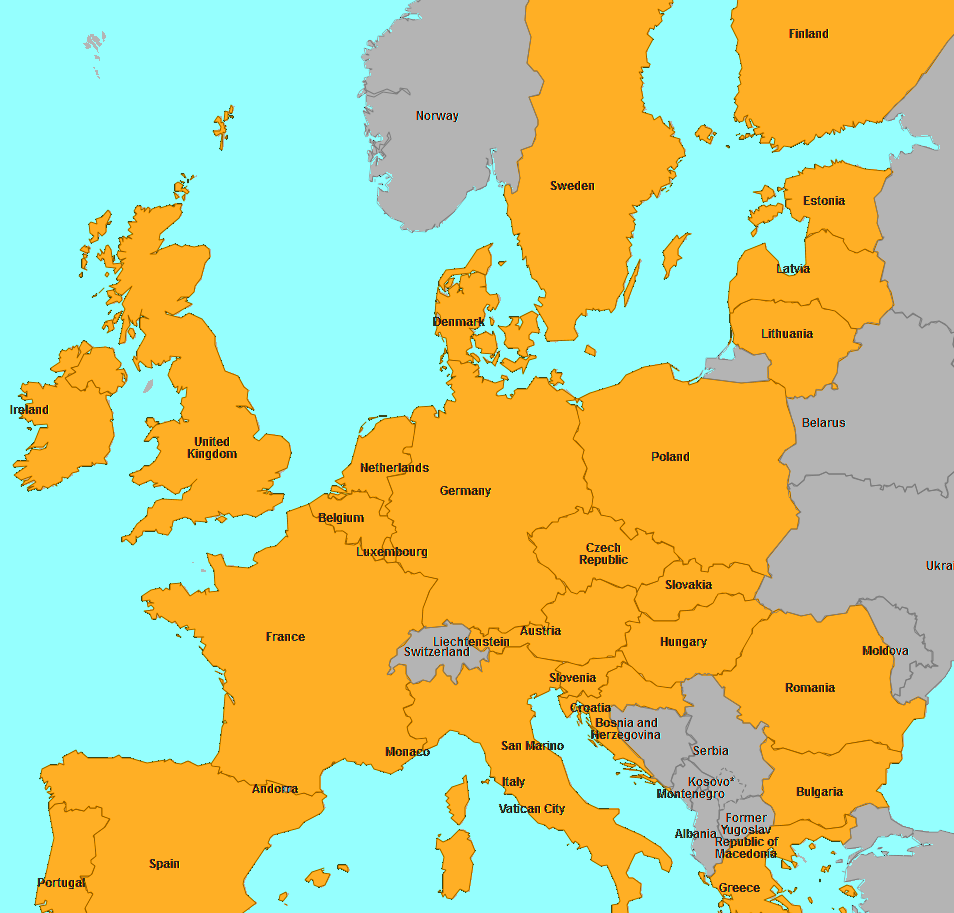
\includegraphics[width=0.6\linewidth]{obr01_EUmapa.png}\end{tabular} & \tiny \begin{tabular}{l l}
			\textbf{EU members:}& \\
			Austria,& Italy,\\
			Belgium,& Latvia,\\
			Bulgaria,& Lithuania,\\
			Croatia,& Luxembourg,\\
			Cyprus,& Malta,\\
			Czech Republic,& Netherlands,\\
			Denmark,& Poland,\\
			Estonia,& Portugal,\\
			Finland,& Romania,\\
			France,& Slovakia,\\
			Germany,& Slovenia,\\
			Greece,& Spain,\\
			Hungary,& Sweden,\\
			Ireland,& United Kingdom\\
		\end{tabular}
		
		\end{tabular}
		\end{center}
	\end{frame}
%------------------------------------------------------------------------------
	\begin{frame}
    \frametitle{Documents}
		\small
		\begin{center}
			\begin{tabular}{m{0.4\linewidth} m{0.5\linewidth}}
			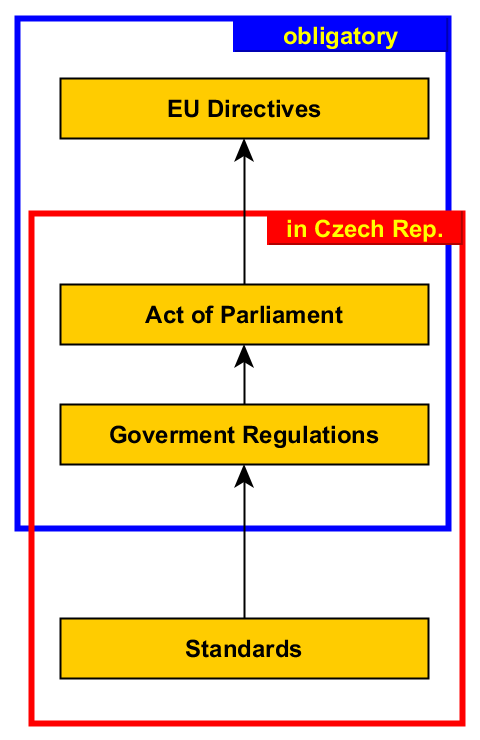
\includegraphics[scale=0.25]{obr02_dokumenty.png} &
			
			\begin{itemize}
				\item EU Directives are obligatory for all EU members,
				\item each country includes the directives in its legal system,
				\item the act of parliament (laws) and government regulations fulfill this task in the legal system of Czech Republic,
				\item the standards are considered as recommendation (not obligatory) in Czech Republic,
			\end{itemize}
			\end{tabular}
		\end{center}
	\end{frame}
%------------------------------------------------------------------------------
	\begin{frame}
    \frametitle{Documents}
		\small
		\begin{center}
			\begin{tabular}{m{0.4\linewidth} m{0.5\linewidth}}
			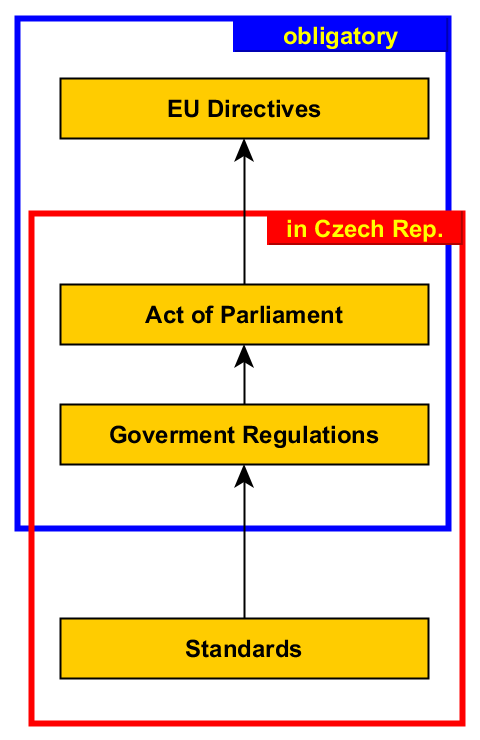
\includegraphics[scale=0.25]{obr02_dokumenty.png} &
			
			\begin{itemize}
				\item \textcolor{blue}{meeting standards requirements is an assumption for meeting Directive requirements},
				\item a product fulfilling the directive requirements is marked by CE symbol and the declaration of conformity is released.
			\end{itemize}
			\end{tabular}
		\end{center}
	\end{frame}
%------------------------------------------------------------------------------
	\begin{frame}
    \frametitle{CE Mark}
		\textbf{The symbol is defined in regulation ES 765/2008, which is complementary to Decision No. 768/2008/EC on a common framework for the marketing of products:}
		\begin{center}
			
\includegraphics[scale=0.45]{obr03_ZnShodyCE.png} 
		\end{center}
	\end{frame}
%------------------------------------------------------------------------------	
	\begin{frame}
    \frametitle{Declaration of Conformity Content - Decision 768/2008/EC}
		\small
		\begin{enumerate}
			\item A product identification number (serial number).
			\item The name and address of the manufacturer or his authorized representative;
			\item \textbf{This declaration of conformity is issued under the sole responsibility of the manufacturer (or installer).}
			\item Object of the declaration (identification of product allowing traceability. It may include a photograph, where
appropriate);
			\item \textbf{The object of the declaration described above is in conformity with the relevant Community harmonization
legislation:} List of directives
		\end{enumerate}

	\end{frame}
%------------------------------------------------------------------------------	
	\begin{frame}
    \frametitle{Declaration of Conformity Content - Decision 768/2008/EC}
		\small
		\begin{enumerate}
			\setcounter{enumi}{5}
			\item References to the relevant harmonized standards used or references to the specifications in relation to which
conformity is declared.
			\item Where applicable, the notified body... (name, number)... performed... (description of intervention)... and issued the certificate.
			\item Additional information.
		\end{enumerate}
		
		\begin{flushright}
		Signed for and on behalf of: ............................
		\end{flushright}
	\end{frame}
%------------------------------------------------------------------------------	
	\begin{frame}
    \frametitle{Declaration of Conformity Example}
		
		\begin{center}
				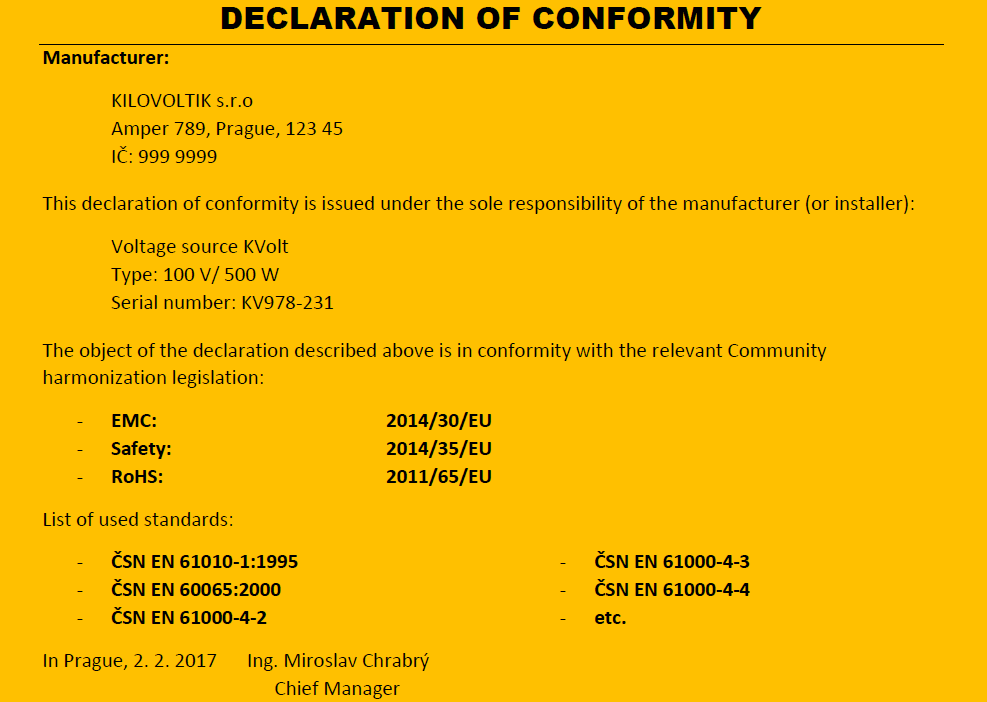
\includegraphics[scale=0.35]{obr04_prohlaseniES.png}
		\end{center}
	\end{frame}
%------------------------------------------------------------------------------	
	\begin{frame}
    \frametitle{Notes}
		
		\begin{itemize}
			\item Products fulfilling requirements of EU directives are free to move across EU market.
			\item Test results from notified laboratory (notified body) are acknowledged in all member countries.
			\item Producer is responsible for his products. He must elaborate technical documentation and record complaints.
		\end{itemize}
	\end{frame}
%------------------------------------------------------------------------------
%Motivation 
%------------------------------------------------------------------------------
\section{\texorpdfstring{Motivation}{Motivation}}
%------------------------------------------------------------------------------
	\begin{frame}
    \frametitle{Problems of Electronic and Electrical Waste}

	\end{frame}
%------------------------------------------------------------------------------
%Legislation
%------------------------------------------------------------------------------
\section{\texorpdfstring{Legislation}{Legislation}}
%------------------------------------------------------------------------------
	\begin{frame}
    \frametitle{Law no. 185/2001 Sb.}
		\small
		\textbf{Czech law about wasted materials: no. 185/2001 Sb.}
		
		\begin{itemize}
			\item It processes several EU directives about wasted materials handling.
			\begin{itemize}
				\item (\textbf{RoHS1}) 2002/95/ES Restriction of the use of certain Hazardous Substances in electrical and electronic equipment
			\end{itemize}
			\item Implementation is ensured via specific \uv{Government Regulations}.
			\item It covers responsibilities, waste sorting, fines, waste treatment etc.
		\end{itemize}
	\end{frame}
%------------------------------------------------------------------------------
	\begin{frame}
    \frametitle{Law no. 185/2001 Sb.}
		\small
		\begin{itemize}
			\item \textbf{Wasted Electronic and Electrical Equipment (\textbf{WEEE})}\\
			\begin{myDef}
			\uv{is product, which functionality depends on electrical current or on electromagnetic filed, or which is determinate for production, transport, measuring of electrical current or electromagnetic filed. It is dedicated for all equipments supplied from 1000 VAC up to 1500 VDC.}
			\end{myDef}
			\item WEEE - all household products are considered as WEEE after finishing their life-time.
		\end{itemize}
		
	\end{frame}
%------------------------------------------------------------------------------
	\begin{frame}
    \frametitle{Law no. 22/1997 Sb.}
		\small
		\textbf{Czech law about technical requirements for products: no. 22/1997 Sb.}
		\begin{itemize}
			\item It considers the requirements for devices released to the market.
			\item Several EU Directives are covered via \uv{Government Regulations}
			\begin{myDef}
			\begin{itemize}
				\item GR no. \textcolor{blue}{86/2011 Sb.} about technical requirements of toys (\textcolor{blue}{Directive 2009/48/ES}),
				\item GR no. \textcolor{blue}{54/2015 Sb.} about technical requirements of medical care equipment (\textcolor{blue}{Directives 93/42/EHS, updated in 98/79/ES, updated in 2000/70/ES, ..., updated in 2007/47/ES}),
				\item ...,
				\item \textcolor{blue}{\textbf{GR no. 481/2012 about restricted use of dangerous materials in electric devices}.}
			\end{itemize}
			\end{myDef}
		\end{itemize}
		
	\end{frame}
	
%------------------------------------------------------------------------------
	\begin{frame}
    \frametitle{Directive 2011/65/ES RoHS}
		\small
		\textbf{(\textbf{RoHS2}) 2011/65/ES Restriction of the use of certain Hazardous Substances in electrical and electronic equipment}
			
			\begin{itemize}
				\item It is covered by GR no. 481/2012 Sb. in Czech Republic
				\item Restricted materials:
				\begin{center}
				\begin{tabular}{|m{0.1\linewidth} |m{0.25\linewidth} |m{0.25\linewidth} |}
				\hline
				& Substance & Concentration\\
				\hline
				Pb & Lead & 0,1 \%\\
				Hg & Mercury & 0,1 \%\\
				Cd & Cadmium & 0,01 \%\\
				Cr & Hexavalent chromium & 0,1 \%\\
				PBB & Polybrominated biphenyls & 0,1 \%\\
				PBDE & Polybrominated diphenyl ethers & 0,1 \%\\
				\hline
				\end{tabular}
			\end{center}
			\end{itemize}
	\end{frame}
%------------------------------------------------------------------------------
	\begin{frame}
    \frametitle{Directive 2011/65/ES RoHS, Consequences}
			\begin{itemize}
				\item There is a lot of exceptions in the directive:
				
				\begin{itemize}
					\item \textbf{Hg} in fluorescent tube,
					\item \textbf{Pb} in fluorescent tube glass, as an alloying element  in steels, in some solders for specific use,
					\item \textbf{Cd} in LEDs, ...
				\end{itemize}
				\item Soldering - just Pb and Cd-free !!! (higher temperature, lower reliability, no advantages)
			\end{itemize}
	\end{frame}
%------------------------------------------------------------------------------
\end{document}